\chapter{Projekt systemu}
\vspace{-25pt}
\section{Opis architektury systemu}
Gra polega na wyświetleniu synthesii wybranej piosenki i zliczaniu punktów zdobywanych przez poprawne powtarzanie sekwencji, która uzyskiwana jest z pliku midi, bądź wyznaczana przez algorytm. Diagram (Rys. 3.1.) przedstawia połączenia pomiędzy pojedynczymi plikami spełniającymi założenia projektu. Strzałkami przerywanymi została zaznaczona część testowa, która pozwalała na ręczne wprowadzanie danych z keyboardu, użytkownik nie będzie korzystał z tej części.

\begin{figure}[h]
  \centering
  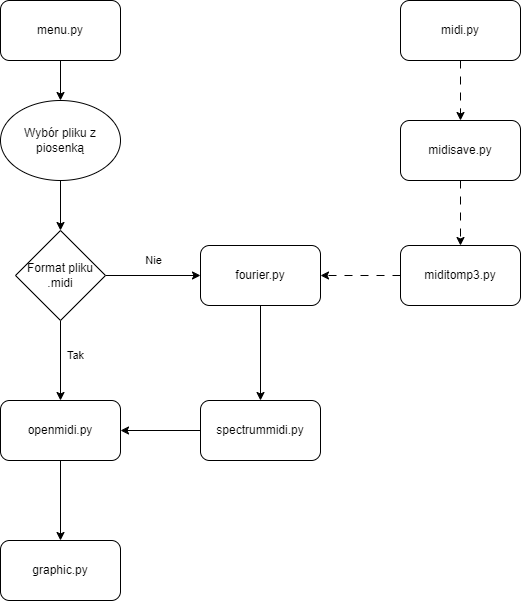
\includegraphics[width=0.69\textwidth]{img/3/diag.png}
  \caption{Diagram przedstawiający architekturę programu}
\end{figure}

\noindent\textbf{Przygotowanie ścieżki dźwiękowej do analizy}

Pierwszym etapem jest odpowiednie przygotowanie ścieżki audio, aby móc przeprowadzić dokładną analizę dźwięku. Najważniejszym elementem przy analizie dźwięku jest widmo ścieżki audio, do którego uzyskania niezbędne jest użycie transformaty Fouriera, a dokładniej STFT. Dzięki czemu można uzyskać macierz amplitud występujących częstotliwości w określonym położeniu w czasie co pozwala na rozpoczęcie analizy ścieżki dźwiękowej.

\begin{figure}[h]
  \centering
  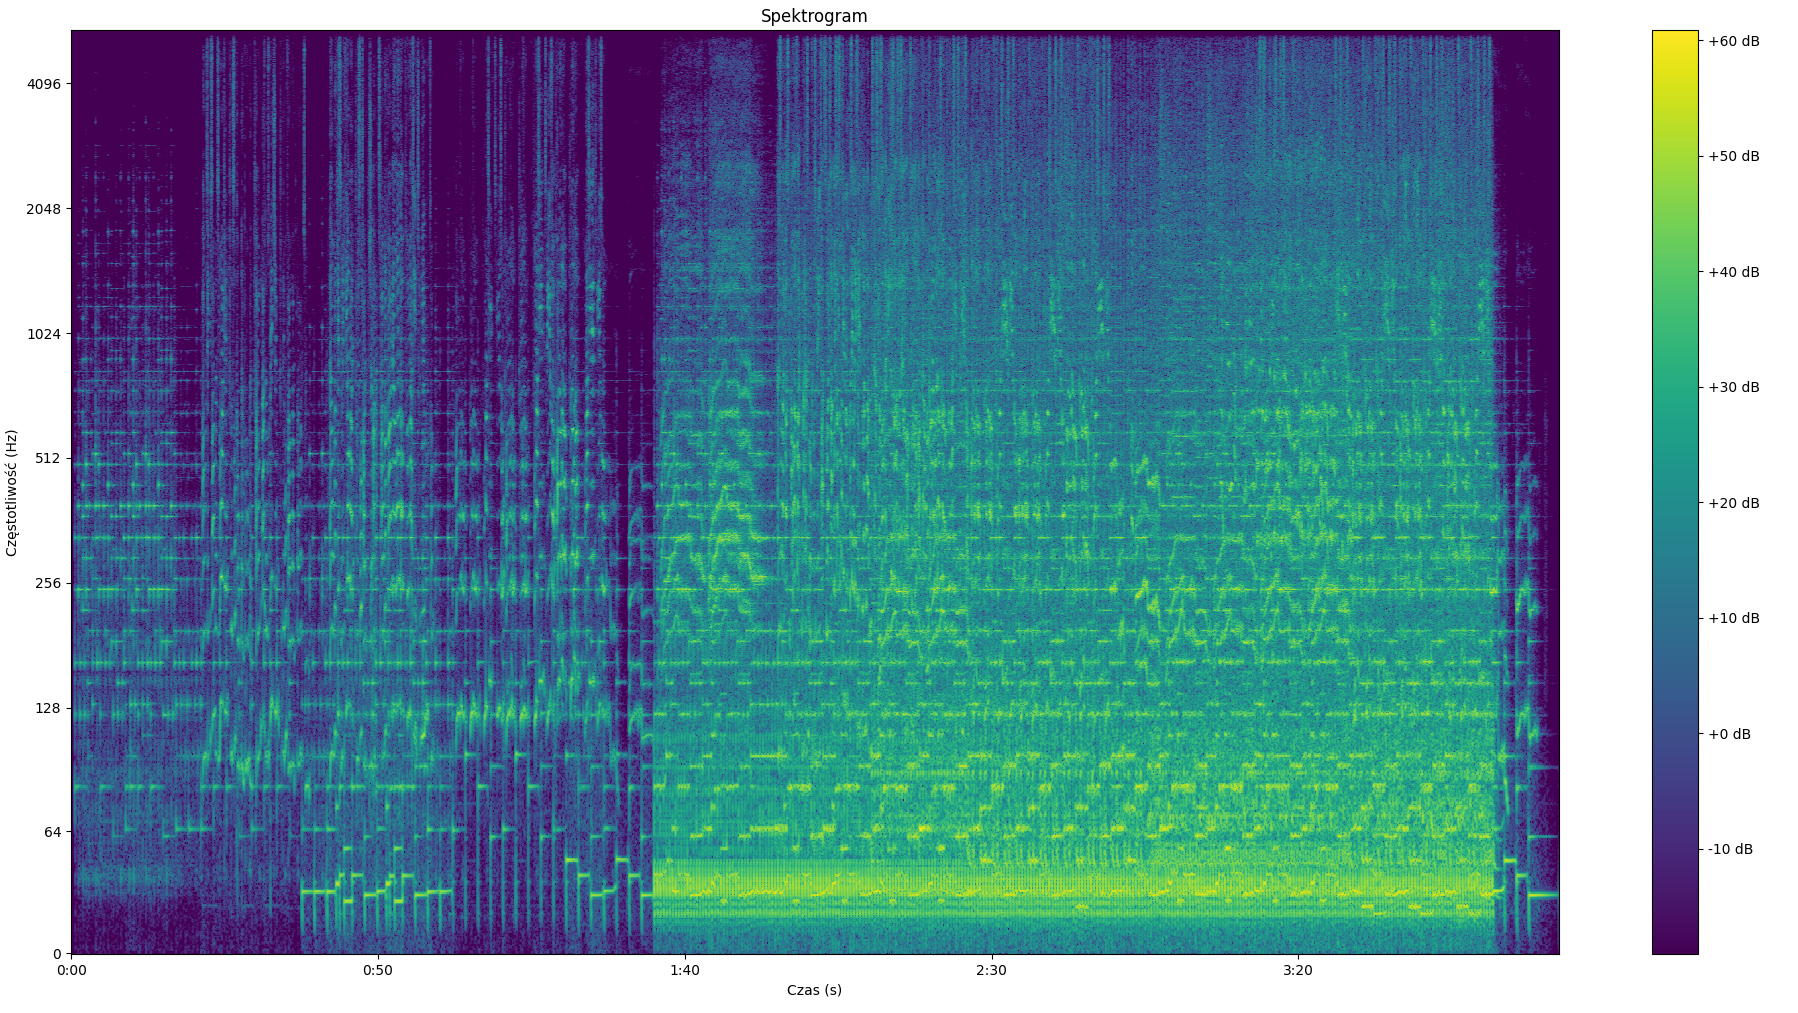
\includegraphics[width=1\textwidth]{img/3/widmo.png}
  \caption{Wykres przedstawiający widmo piosenki Tom Odell - Another Love}
\end{figure}

\noindent\textbf{Synteza dźwięku}

Dźwięk jest tworzony za pomocą syntezy wavetable, ponieważ jest to prosty sposób oraz najbardziej zbliżony do syntezy dźwięku w keyboardzie, gdzie zazwyczaj stosowana jest synteza próbkowa, która odtwarza dźwięki wcześniej nagranych instrumentów. Używając syntezy wavetable, ton zawarty w formacie midi jest podstawiany do gotowych cyfrowych tabel i odpowiednio głośny zależnie od wysokości amplitudy.\\


\noindent\textbf{Interfejs użytkownika}

Użytkownik po uruchomieniu gry ujrzy menu, w którym ma do wyboru rozpoczęcie gry oraz ustawienia. Wciśnięcie przycisku Start powoduje możliwość wyboru pliku audio w formacie mp3/wav, a następnie w tle zostanie przeliczony na plik midi. Zostanie rozpoczęte wyświetlanie grafiki oraz naliczanie punktów na podstawie poprawnego odtwarzania wyświetlanych klawiszy.

\section{Wybór narzędzi i technologii do implementacji}

Za narzędzia posłużył keyboard marki CASIO model CTK-496 \cite{casio_ctk496} oraz interfejs audio MIDI USB marki Roland model UM-ONE MK2 \cite{roland_um_one}, za pomocą których analizowano widmo częstotliwościowe, testowano działanie konwersji na format midi oraz odbieranie sygnału wraz z przeliczaniem punktów uzyskiwanych za poprawne wciskanie klawiszy.

Program został zaprojektowany na system Windows ze względu na jego powszechność wśród użytkowników. Zaimplementowany został w języku Python\cite{python} ze względu na ogrom dostępnych bibliotek oraz ze względu na możliwości w przetwarzaniu dużej ilości danych.

\subsection{Biblioteki Python}

\noindent\textbf{Numpy}\cite{numpy}

To biblioteka do obliczeń numerycznych. Zapewnia efektywne operacje na macierzach, tablicach oraz funkcje matematyczne, umożliwiając pracę z danymi numerycznymi.\\

\noindent\textbf{LibROSA}\cite{librosa}

Jest to biblioteka do analizy sygnałów audio. Umożliwia wczytywanie, przetwarzanie i analizę danych dźwiękowych, oferując narzędzia do ekstrakcji cech dźwiękowych i tworzenia reprezentacji sygnałów. Dostarcza również narzędzia do wizualizacji danych dźwiękowych, umożliwiając wygodne tworzenie wykresów i reprezentacji graficznych sygnałów.\\

\noindent\textbf{Matplotlib}\cite{matplotlib}

Biblioteka służąca do tworzenia wykresów, grafik i wizualizacji danych. Jest często wykorzystywana w analizie danych, naukowych wizualizacjach oraz prezentacji danych ze względu na swoją elastyczność i możliwości dostosowywania wykresów.\\

\noindent\textbf{Pygame}\cite{pygame}

Biblioteka do tworzenia gier i aplikacji multimedialnych. Zawiera moduły do obsługi grafiki, dźwięku, interakcji z użytkownikiem i innych aspektów tworzenia gier.\\

\noindent\textbf{pygame menu}\cite{pygame_menu}

Jest to moduł rozszerzający bibliotekę Pygame, umożliwiający łatwe tworzenie interfejsów użytkownika dla gier i aplikacji napisanych w Pygame.

\newpage
\noindent\textbf{Mido}\cite{mido}

Biblioteka do obsługi danych MIDI. Umożliwia odczyt, zapis, manipulację i tworzenie plików MIDI oraz interakcję z urządzeniami obsługującymi protokół MIDI.\\

\noindent\textbf{midi2audio}\cite{midi2audio}

To narzędzie, które konwertuje pliki MIDI na pliki dźwiękowe (np. WAV, MP3). Używa biblioteki FluidSynth do generowania dźwięku na podstawie plików MIDI.\\

\noindent\textbf{Threading}\cite{threading}

Moduł Pythona umożliwiający tworzenie wielowątkowych aplikacji, gdzie wątki działają równolegle, przydatne do operacji nieblokujących.\\

\noindent\textbf{Tkinter}\cite{tkinter}

Moduł Pythona zawierający standardowy pakiet do tworzenia interfejsów graficznych użytkownika (GUI), oferujący narzędzia do tworzenia okien, przycisków i innych elementów interfejsu.\\

\noindent\textbf{sys}\cite{sys}

Moduł Pythona zapewniający dostęp do niektórych zmiennych i funkcji interakcji ze środowiskiem systemu.\\

\noindent\textbf{os}\cite{os}

Moduł Pythona dostarczający funkcje do interakcji z systemem operacyjnym, takie jak manipulacja plikami, tworzenie katalogów itp.

\subsection{Dodatkowe narzędzia}

\noindent\textbf{FluidSynth }\cite{fluidsynth}

FluidSynth to syntezator dźwięku, który używa plików SoundFont do generowania dźwięku na podstawie plików MIDI. Pliki SoundFont zawierają próbki dźwiękowe różnych instrumentów muzycznych oraz informacje dotyczące sposobu ich odtwarzania. FluidSynth jest narzędziem open-source, które umożliwia odczyt plików MIDI i syntezę dźwięku na ich podstawie. Dzięki temu użytkownik może generować dźwięki różnych instrumentów muzycznych, manipulować parametrami dźwięku, takimi jak wibrato, głośność czy barwa, co jest przydatne w procesie komponowania, edycji dźwięku czy też w aplikacjach muzycznych.

\newpage

\noindent\textbf{FFmpeg} \cite{ffmpeg}

FFmpeg to zestaw narzędzi do nagrywania, konwersji i strumieniowania plików audio oraz wideo. Jest to oprogramowanie open-source, które działa na wielu platformach, umożliwiając manipulację multimediów. Za jego pomocą można wykonywać różne operacje, takie jak konwersja formatów plików, kompresja, ekstrakcja strumieni wideo i audio, łączenie plików, nagrywanie strumieni czy też aplikowanie efektów. FFmpeg obsługuje dużą liczbę formatów plików multimedialnych i oferuje szeroki zakres opcji konfiguracyjnych, co sprawia, że jest powszechnie używany w edycji wideo i audio, transmisji strumieniowej, produkcji multimediów oraz jako silnik w wielu aplikacjach multimedialnych.

\section{Algorytm}

\subsection{Analiza ścieżki dźwiękowej}

Wykres spektrogramu ukazuje dominujące częstotliwości oraz ich położenie, natomiast oprócz samych głównych dźwięków widoczna jest ich powtarzalność z oktawy na oktawę wraz ze wzrostem częstotliwości. Są to składowe harmoniczne, które nadają dźwięku charakterystyczną barwę oraz głębię. Dzięki nim piosenka staje się bogatsza oraz sprawiają, że analiza dźwięku jest znacznie cięższa. Powodem tego jest ich zróżnicowanie, co uniemożliwia ich jednoznaczną identyfikację. Możliwe jest również powielenie się składowych harmonicznych z głównym dźwiękiem, co powoduje że główny dźwięk może zostać uznany jako składowa harmoniczna i nie zostać wykryty.
\subsection{Detekcja tonów}

\noindent\textbf{Główne założenia detekcji}

Ton może zostać wykryty za pomocą tylko jednej zmiennej, mianowicie amplitudy, a każdemu z nich odpowiada konkretna częstotliwość (Tab. 2.1). Rozpoznawanie dźwięków rozpocznie się od przechodzenia po kolei każdej zdefiniowanej w tabeli częstotliwości po czasie. Miejsca, w których amplituda jest odpowiednio wysoka oznacza znalezienie poszukiwanego tonu. Algorytm początkowo poszukuje komórki, gdzie amplituda osiągnie maksimum lokalne, którego wartość jest większa od ustalonego progu detekcji. Następnie cofa się w czasie, aż do znalezienia minimum lokalnego, co oznacza wykrycie rozpoczęcia się danego dźwięku. Po tym algorytm idzie dalej od maksimum lokalnego szukając minimum lokalnego. Jeśli zostanie znalezione, a amplituda nadal będzie wyższa niż ustalony próg, to oznacza znalezienie miejsca, w którym ten sam klawisz został ponownie naciśnięty i rozpoczął się ponowny wzrost amplitudy w czasie. Natomiast jeśli minimum nie zostało znalezione, zanim amplituda przekroczyła granicę podtrzymania tonu, zostaje zapisana informacja o zakończeniu wciśnięcia danego dźwięku.\\




\noindent\textbf{Próg graniczny detekcji}

Wnioskując z uprzednich założeń, wykrywanie tonów zależy głównie od ustalonej wartości progu detekcji. Do jego ustalenia potrzebny jest zakres amplitud, jaki występuje w danej ścieżce muzycznej. Próg należało dobrać tak, aby zostały wykryte tony występujące w danym utworze, a nie zostały wykryte żadne, które w nim nie występują. 

Pierwsza metoda wyznaczania progu wykonuje to z użyciem wartości maksymalnej amplitudy pomnożonej przez współczynnik ustalony w zależności od charakterystyki utworu. 
Jednakże piosenki nie są jednostajne, składają się z fragmentów, gdzie wahania amplitudy dźwięków są względnie stałe, jak i również z fragmentów wyciszenia oraz nasilenia. 

Uwzględniając to powstała druga metoda wyznaczając próg detekcji używając maksymalnej amplitudy oraz średniej, które zostały zsumowane i wymnożone przez współczynniki.

Niemniej jednak w zależności od barwy oraz charakterystyki utworu dźwięki różnią się amplitudą nie tylko na przestrzeni czasu, ale również częstotliwości. Metoda trzecia zatem odzwierciedla szukanie tonów przez człowieka na wykresie widma, czyli doszukiwanie się poziomych linii o wyższej amplitudzie niż najbliższe otoczenie. Otoczenie w zakresie częstotliwości, będzie obejmowało zauważalne zwiększenie amplitudy przez dany ton, a w zakresie czasu kilkaset milisekund.\\

\noindent\textbf{Składowe harmoniczne}

Główną przeszkodą w poprawnym rozpoznawaniu tonów są składowe harmoniczne. Jak zostało wcześniej wspomniane mogą przykryć główny dźwięk, bądź go imitować. 

Składowe harmoniczne występują na częstotliwościach, które są wielokrotnościami częstotliwości, od której pochodzą i są znacząco widoczne na dwukrotności, trzykrotności oraz czterokrotności tejże częstotliwości. Dwukrotność oraz czterokrotność nie zmienia drastycznie wybrzmienia, ponieważ to jest ten sam ton tylko oktawę i dwie oktawy wyżej, czyli dwanaście i dwadzieścia cztery półtony. Natomiast trzykrotność częstotliwości znacząco może zmienić brzmienie, ponieważ przykładowo dźwięk A na drugiej oktawie ma częstotliwość 110Hz. Trzykrotność tej częstotliwości to 330Hz, która jest na tyle blisko dźwięku E na czwartej oktawie (którego częstotliwość wynosi 329.63Hz), że znacząco wpływa na podwyższenie amplitudy i może powodować że dźwięk może zostać błędnie zidentyfikowany. Błąd między harmoniczną trzykrotną, a najbliższym tonem to zaledwie około jeden procent błędu względem kolejnego tonu. 

Niestety wiele utworów muzycznych składa się z sekwencji, gdzie grany ton jest grany również o dwanaście, dziewiętnaście i dwadzieścia cztery półtony. Dźwięki harmoniczne również nie mają zależności w postaci amplitudy, czasem potrafią mieć większy poziom decybeli, niż dźwięk z którego pochodzą, a więc nie ma żadnej zasady, którą byłaby możliwość kierowania się, a co za tym idzie próbując usunąć składowe harmoniczne, najprawdopodobniej zostaną usunięte główne dźwięki.

Próba usunięcia dźwięków harmonicznych polega na sprawdzaniu przy każdym znalezionym dźwięku, czy w bardzo małym zakresie przed jego rozpoczęciem, nie rozpoczął się dźwięk niższy o dwanaście, dziewiętnaście i dwadzieścia cztery półtony.
